% OsdagBridge Project Management Handbook
% Build: bash build.sh   (runs pdflatex twice)
% Toolchain: pdflatex (TeX Live). No shell-escape, no external fonts.
\documentclass[11pt,a4paper]{report}

\usepackage[T1]{fontenc}
\usepackage[utf8]{inputenc}
\usepackage{lmodern}
\usepackage[a4paper,margin=1in]{geometry}
\usepackage{microtype}
\usepackage{parskip}
\usepackage{xcolor}
\usepackage{booktabs}
\usepackage{longtable}
\usepackage{array}
\usepackage{enumitem}
\usepackage{needspace}
\usepackage{titlesec}
\usepackage{fancyhdr}
\usepackage{listings}
\usepackage{tikz}
\usetikzlibrary{positioning,arrows.meta,shapes.geometric,chains,fit,backgrounds}
\usepackage[most]{tcolorbox}
\usepackage[hidelinks]{hyperref}

% ---- palette ---------------------------------------------------------------
\definecolor{ink}{HTML}{16213E}
\definecolor{brandblue}{HTML}{1F6FEB}
\definecolor{peGreen}{HTML}{1B7F4B}
\definecolor{peGreenBg}{HTML}{EAF7EF}
\definecolor{gotchaRed}{HTML}{B4232A}
\definecolor{gotchaBg}{HTML}{FCEDED}
\definecolor{verifyBlue}{HTML}{0B5FA5}
\definecolor{verifyBg}{HTML}{EAF2FB}
\definecolor{noteGray}{HTML}{4A4A4A}
\definecolor{noteBg}{HTML}{F1F1F1}
\definecolor{codebg}{HTML}{F6F8FA}
\definecolor{rulegray}{HTML}{D0D0D0}

\hypersetup{
  colorlinks=true, linkcolor=brandblue, urlcolor=brandblue, citecolor=brandblue,
  pdftitle={OsdagBridge Project Management Handbook},
  pdfauthor={OsdagBridge PM}, bookmarksnumbered=true
}

% ---- headings --------------------------------------------------------------
\titleformat{\chapter}[display]
  {\normalfont\huge\bfseries\color{ink}}
  {\color{brandblue}\large\MakeUppercase{\chaptertitlename}\ \thechapter}{6pt}{\Huge}
\titlespacing*{\chapter}{0pt}{0pt}{20pt}

\pagestyle{fancy}
\fancyhf{}
\fancyhead[L]{\small\itshape OsdagBridge PM Handbook}
\fancyhead[R]{\small\thepage}
\renewcommand{\headrulewidth}{0.4pt}
\renewcommand{\footrulewidth}{0pt}

\setcounter{tocdepth}{1}
\setcounter{secnumdepth}{2}

% ---- callout boxes ---------------------------------------------------------
\newtcolorbox{plainenglish}{breakable,enhanced,colback=peGreenBg,colframe=peGreen,
  coltitle=white,fonttitle=\bfseries,title=In plain English,
  left=2.5mm,right=2.5mm,top=1.4mm,bottom=1.4mm,boxrule=0.7pt,arc=1.5mm}
\newtcolorbox{gotcha}{breakable,enhanced,colback=gotchaBg,colframe=gotchaRed,
  coltitle=white,fonttitle=\bfseries,title=Open-source gotcha,
  left=2.5mm,right=2.5mm,top=1.4mm,bottom=1.4mm,boxrule=0.7pt,arc=1.5mm}
\newtcolorbox{verifybox}{breakable,enhanced,colback=verifyBg,colframe=verifyBlue,
  coltitle=white,fonttitle=\bfseries,title=Check it worked,
  left=2.5mm,right=2.5mm,top=1.4mm,bottom=1.4mm,boxrule=0.7pt,arc=1.5mm}
\newtcolorbox{notebox}{breakable,enhanced,colback=noteBg,colframe=noteGray,
  coltitle=white,fonttitle=\bfseries,title=Note,
  left=2.5mm,right=2.5mm,top=1.4mm,bottom=1.4mm,boxrule=0.7pt,arc=1.5mm}

% ---- code listings ---------------------------------------------------------
\lstdefinestyle{clicks}{basicstyle=\ttfamily\small,backgroundcolor=\color{codebg},
  frame=single,rulecolor=\color{rulegray},framerule=0.4pt,breaklines=true,
  columns=fullflexible,keepspaces=true,xleftmargin=3mm,xrightmargin=1mm,
  aboveskip=7pt,belowskip=7pt,literate={->}{{$\rightarrow$}}1 {→}{{$\rightarrow$}}1}
\lstset{style=clicks}

\newcommand{\code}[1]{\texttt{#1}}
\newcommand{\fieldname}[1]{\textbf{#1}}

% ===========================================================================
\begin{document}

% ---- title page ------------------------------------------------------------
\begin{titlepage}
\centering
\vspace*{2.2cm}
{\color{brandblue}\rule{\textwidth}{2pt}}\\[10pt]
{\Huge\bfseries\color{ink} OsdagBridge}\\[6pt]
{\Huge\bfseries\color{ink} Project Management Handbook}\\[14pt]
{\large A start-from-zero guide to the board, epics, and sprints.}\\[6pt]
{\color{brandblue}\rule{\textwidth}{2pt}}\\[26pt]

\begin{minipage}{0.82\textwidth}\centering\itshape
If you have never run a project board, never heard the word ``epic,'' and are not
sure what a ``sprint'' has to do with software, this book is written for you.
Read it front to back once. After that, keep it next to the board.
\end{minipage}

\vfill
{\large Version 1.1 \quad|\quad 1 August 2026}\\[4pt]
{\small Part of \textbf{Osdag Project Management} --- one engine, many FOSSEE-project boards.}\\[2pt]
{\small Repository: \code{nishikantmandal007/Osdag-Project-Management}}\\[2pt]
{\small Board: project \#3, ``OsdagBridge''}
\vspace*{1.5cm}
\end{titlepage}

\tableofcontents
\thispagestyle{empty}
\cleardoublepage

% ---- foreword --------------------------------------------------------------
\chapter*{Before you start}
\addcontentsline{toc}{chapter}{Before you start}

\textbf{Who this is for.} New contributors and interns joining OsdagBridge, and
anyone who has to keep the project board honest. No project-management background
is assumed. Every term is defined the first time it appears.

\textbf{How the book is laid out.}

\begin{itemize}[leftmargin=1.4em,itemsep=2pt]
  \item \textbf{Part I} teaches project management from scratch, with plain
        analogies. Read this if words like \emph{epic}, \emph{backlog}, or
        \emph{triage} are new to you.
  \item \textbf{Part II} maps those ideas onto OsdagBridge specifically: our
        labels, our ten epics, our bug tiers.
  \item \textbf{Part III} walks you through building the board from an empty
        page, one field and one view at a time.
  \item \textbf{Part IV} is the daily and fortnightly routine: how a sprint runs
        and how one issue travels from ``someone reported it'' to ``done.''
  \item \textbf{Part V} answers three questions people always ask about running a
        board in the open: can outsiders break it, how do interns join without
        repository access, and were all those robots really necessary.
  \item \textbf{Part VI} is reference material: a glossary, a map of which
        configuration file controls what, and a one-page cheat sheet.
\end{itemize}

\begin{notebox}
This handbook is the friendly, long-form guide. The short checklists it is based
on live next to it as \code{SOP-01} through \code{SOP-10} and
\code{BOARD-SETUP.md}. When this book says ``see the triage SOP,'' it means one of
those files. You never need them to follow along here, but they are the terse
reference once you know the ropes.
\end{notebox}

% ===========================================================================
\part{Project Management from Zero}

\chapter{Why a project needs a ``management layer''}

OsdagBridge is real engineering software. It sizes and checks steel bridges. About
ten people have written roughly ninety thousand lines of Python over a thousand
commits. That is a serious amount of work by a serious group of people.

For a long time the way that work got tracked was a single long list of tickets on
GitHub. Ninety-three of them, open at once. No order beyond newest-on-top. No way
to tell a wrong-answer bug from a spelling mistake. No way to see who was doing
what, or which tickets belonged together, or what had to ship before a release. A
majority of them had nobody's name on them at all.

That list is not a failure. It is what every growing project produces if nothing
organises the incoming work. The pile just grows until people stop being able to
see the shape of it.

\begin{plainenglish}
A ``project management layer'' is not extra bureaucracy on top of the real work.
It is the difference between a kitchen during a dinner rush with tickets stuck up
in order, owned by one cook each, and the same kitchen with orders shouted into
the air and everyone hoping someone heard. Same cooks, same food. One of them
serves dinner.
\end{plainenglish}

The goal of this system is not to make people work faster. OsdagBridge's throughput
was already climbing on its own. The goal is three plainer things:

\begin{itemize}[leftmargin=1.4em,itemsep=3pt]
  \item \textbf{Intake discipline.} Every new report gets sorted the same way, so
        nothing rots unseen at the bottom of a list.
  \item \textbf{Ownership.} Every piece of work has one name on it, so ``someone
        should look at this'' becomes ``you are looking at this.''
  \item \textbf{Traceability.} You can follow any result on screen back to the
        line of code and the test that guards it. For structural software, where
        a wrong number can be an unsafe bridge, this is the whole point.
\end{itemize}

\chapter{The words, with pictures}

Project management has its own vocabulary. None of it is hard once you have a
picture for it. Here is the whole cast.

\section{Issue}
An \textbf{issue} is one unit of work or one conversation. A bug report is an
issue. A feature request is an issue. ``Rename this button'' is an issue. On
GitHub, an issue has a number (\code{\#42}), a title, a description, labels, and
one or more people assigned to it. Everything else in this chapter is a way of
grouping, sorting, or scheduling issues.

\section{The work-item hierarchy: Release, Epic, Story, Task}

Work comes in sizes. A one-line typo fix and ``make every result on screen
traceable to its source'' are both ``work,'' but pretending they are the same size
helps nobody. So we stack work in four layers.

\begin{plainenglish}
Think of a book.
\textbf{An epic is the book} (``result traceability'').
\textbf{A story or a bug is a chapter} (``the shear result disagrees between the
screen and the report'').
\textbf{A task is a paragraph} (``add a test that pins the shear number'').
And \textbf{a release is the shelf} the finished books ship on together
(``version 1.0'').
You read a book chapter by chapter. You finish an epic issue by issue.
\end{plainenglish}

\begin{center}
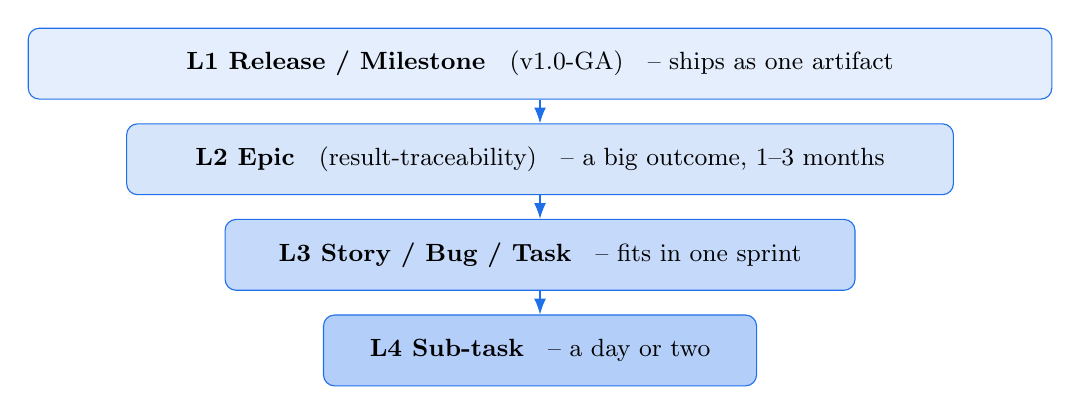
\begin{tikzpicture}[font=\small,node distance=0pt]
  \node[draw=brandblue,fill=brandblue!12,rounded corners,minimum width=13cm,minimum height=0.9cm] (r) {\textbf{L1 Release / Milestone} \; (v1.0-GA) \; -- ships as one artifact};
  \node[draw=brandblue,fill=brandblue!18,rounded corners,minimum width=10.5cm,minimum height=0.9cm,below=3mm of r] (e) {\textbf{L2 Epic} \; (result-traceability) \; -- a big outcome, 1--3 months};
  \node[draw=brandblue,fill=brandblue!26,rounded corners,minimum width=8cm,minimum height=0.9cm,below=3mm of e] (s) {\textbf{L3 Story / Bug / Task} \; -- fits in one sprint};
  \node[draw=brandblue,fill=brandblue!34,rounded corners,minimum width=5.5cm,minimum height=0.9cm,below=3mm of s] (t) {\textbf{L4 Sub-task} \; -- a day or two};
  \draw[-{Latex[length=2mm]},brandblue] (r.south) -- (e.north);
  \draw[-{Latex[length=2mm]},brandblue] (e.south) -- (s.north);
  \draw[-{Latex[length=2mm]},brandblue] (s.south) -- (t.north);
\end{tikzpicture}
\end{center}

\begin{center}
\begin{tabular}{@{}p{2.3cm}p{4.3cm}p{2.6cm}p{3.2cm}@{}}
\toprule
\textbf{Level} & \textbf{What it is} & \textbf{Lives for} & \textbf{Done when}\\
\midrule
L1 Release & A version you ship (\code{v1.0-GA}) & A quarter or two & Every child epic is done \\
L2 Epic & A large outcome & 1--3 months & The outcome is achieved \\
L3 Story/Bug/Task & One shippable piece & One sprint or less & Merged and verified \\
L4 Sub-task & A checklist item under an issue & A day or two & Checked off \\
\bottomrule
\end{tabular}
\end{center}

A word you will hear: a \textbf{sub-epic}. When an epic is so big it would hold a
hundred child issues, you split it into a few smaller epics. We do this for exactly
one epic today (result-traceability), because it touches the largest slice of the
backlog. More on that in Part II.

\section{Backlog}
The \textbf{backlog} is everything you have agreed is worth doing but have not
scheduled yet. It is the ``soon, or someday'' pile. A healthy backlog is groomed:
old items get re-read, big ones get split, dead ones get closed. An ungroomed
backlog is just the ninety-three-ticket list again.

\section{Sprint}
A \textbf{sprint} is a fixed, short window of time, two weeks for us, in which the
team commits to finishing a chosen handful of issues. The window does not move. If
work does not fit, the work moves to the next sprint, not the deadline.

\begin{plainenglish}
A sprint is a fortnightly promise, not a countdown timer on any one task. On Monday
you pull a stack of issues you believe you can finish by the following Friday week.
Then you protect that stack. The point of the fixed window is rhythm: you always
know when the next planning and the next review happen.
\end{plainenglish}

\section{Board, columns, and Status}
The \textbf{board} is the picture of all your issues as cards, arranged in columns.
The column an issue sits in is its \textbf{Status}. Our columns run left to right
like an assembly line.

\begin{center}
\resizebox{\textwidth}{!}{%
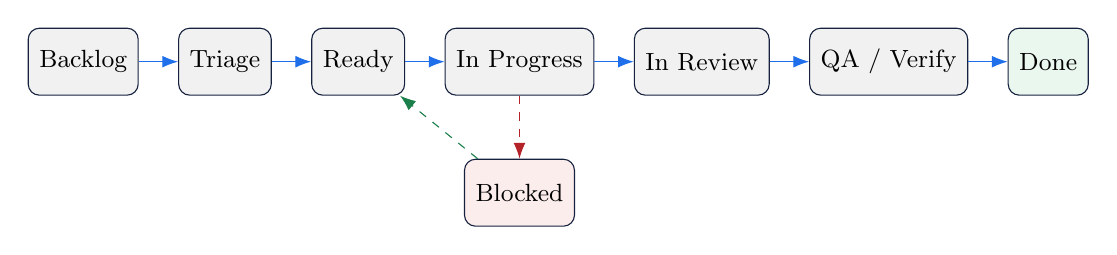
\begin{tikzpicture}[font=\small,>={Latex[length=2mm]}]
  \tikzstyle{st}=[draw=ink,fill=noteBg,rounded corners,minimum height=0.85cm,inner xsep=4pt]
  \node[st] (b) {Backlog};
  \node[st,right=5mm of b] (t) {Triage};
  \node[st,right=5mm of t] (r) {Ready};
  \node[st,right=5mm of r] (p) {In Progress};
  \node[st,right=5mm of p] (v) {In Review};
  \node[st,right=5mm of v] (q) {QA / Verify};
  \node[st,fill=peGreenBg,right=5mm of q] (d) {Done};
  \foreach \a/\c in {b/t,t/r,r/p,p/v,v/q,q/d} \draw[->,brandblue] (\a) -- (\c);
  \node[st,fill=gotchaBg,below=8mm of p] (bl) {Blocked};
  \draw[->,gotchaRed,dashed] (p) -- (bl);
  \draw[->,peGreen,dashed] (bl) -- (r);
\end{tikzpicture}}
\end{center}

\textbf{Blocked} is off to the side on purpose. It is not a stage you pass through,
it is a place a card waits when something outside it is in the way. A blocked card
must name what it is waiting on.

\section{Severity versus Priority}
These two get confused constantly, so pin them down now.

\begin{itemize}[leftmargin=1.4em,itemsep=2pt]
  \item \textbf{Severity} is \emph{how bad the problem is}. A wrong structural
        number shown as if it were right is the worst kind. A misaligned toolbar
        icon is the mildest.
  \item \textbf{Priority} is \emph{how soon we will deal with it}. It is a
        scheduling decision, not a fact about the bug.
\end{itemize}

A tiny cosmetic bug can be high priority the week before a demo. A serious bug can
be low priority if it only affects a feature nobody ships yet. Severity is a
property of the problem; priority is a choice you make.

\section{Points and velocity}
Some teams put a rough size number on each issue (\textbf{story points}: 1, 2, 3,
5, 8) and track how many points they finish per sprint (\textbf{velocity}). It is a
capacity estimate, not a score. We keep the field available but do not lean on it.
Do not treat velocity as a target to maximise; it is a planning aid.

\section{Milestone and Release}
A \textbf{milestone} (or release) is a named finish line that groups issues due for
the same version, like \code{v1.0-GA}. ``GA'' means \emph{general availability}:
the version you would hand to a stranger.

\section{Triage}
\textbf{Triage} is the sorting step every new issue passes through: decide its
type, its severity if it is a bug, which part of the code it touches, and who owns
it. The word comes from hospitals, and the spirit is the same. You are not fixing
anything yet. You are deciding what this is and how urgent it is, quickly, so
nothing waits in the dark.

\chapter{Agile and Scrum, in one page}

You will hear the words \textbf{Agile} and \textbf{Scrum}. Here is all you need.

\textbf{Agile} is a way of working that prefers shipping small, useful increments
often, and adjusting as you learn, over writing one giant plan up front and
following it for a year. \textbf{Scrum} is one popular recipe for doing Agile, and
sprints come from it.

We borrow the useful parts and skip the ceremony.

\begin{center}
\begin{tabular}{@{}p{6.2cm}p{7.2cm}@{}}
\toprule
\textbf{We borrow} & \textbf{We skip} \\
\midrule
Two-week sprints with a planning and a review & Daily stand-up meetings; we are a distributed, part-volunteer team \\
A groomed backlog and clear ownership & Story-point obsession and velocity targets \\
Service-level targets measured in \emph{business days} & Any pretence of a 24/7 on-call rotation \\
A board that shows the true state of the work & Rituals that exist to be performed, not to help \\
\bottomrule
\end{tabular}
\end{center}

\begin{notebox}
When you read that a serious bug should be triaged ``within one business day,''
that means someone looks at it and sorts it within a working day. It does not mean
anyone is paged at 2am. These are promises a volunteer team can actually keep.
\end{notebox}

% ===========================================================================
\part{The OsdagBridge System, Concretely}

\chapter{Our four levels, on our project}

The generic hierarchy from Part~I lands like this on OsdagBridge:

\begin{itemize}[leftmargin=1.4em,itemsep=3pt]
  \item \textbf{Releases} are \code{v1.0-GA}, \code{v1.1}, \code{v2.0}. Most of the
        current work aims at \code{v1.0-GA}.
  \item \textbf{Epics} are the ten big outcomes in the next chapter, tagged
        \code{type:epic}.
  \item \textbf{Stories, bugs, and tasks} are the everyday issues, each tagged with
        a \code{type:}, and for bugs a \code{sev:}, and one or more \code{area:}
        labels.
  \item \textbf{Sub-tasks} are checklist items linked under an issue as native
        GitHub sub-issues.
\end{itemize}

\chapter{Labels: three decisions per issue}

A \textbf{label} is a coloured tag on an issue. We use three families of them, and
the rule is simple: a well-triaged issue answers three questions through its
labels. \emph{What kind of thing is it? If it is a bug, how bad? Which part of the
code?}

\section{\code{type:} what kind of work}
\begin{center}
\begin{tabular}{@{}lp{9.5cm}@{}}
\toprule
\textbf{Label} & \textbf{Meaning} \\
\midrule
\code{type:epic}    & An outcome-level container. Closes when the outcome is achieved. \\
\code{type:feature} & New capability a user asked for. \\
\code{type:story}   & A sprint-sized piece of user value. \\
\code{type:bug}     & Something behaves incorrectly. \\
\code{type:task}    & Sprint-sized work with no direct user story. \\
\code{type:chore}   & Housekeeping (dependencies, cleanup). \\
\code{type:spike}   & A time-boxed investigation to answer a question. \\
\code{type:docs}    & Documentation. \\
\code{type:test}    & A test to be written, often filed by a bot when a bug closes. \\
\bottomrule
\end{tabular}
\end{center}

\section{\code{sev:} how bad the bug is}
Bugs, and only bugs, also get a severity. The four tiers get their own chapter
below because the definitions carry real weight.

\section{\code{area:} which part of the code}
\code{area:} is the subsystem the issue touches, and it is \emph{multi-valued}: an
issue routinely spans two areas, and that is allowed. Examples you will see:
\code{design-core}, \code{analysis-opensees}, \code{reports}, \code{ifc-boq},
\code{packaging}, \code{memory-stability}, \code{ci-cd}, \code{docs}, plus the
user-interface areas carried over from the old tracker.

\begin{notebox}
You may notice the board has fields for \textbf{Priority}, \textbf{Size},
\textbf{Epic}, and \textbf{Target release} too, but there are no \code{pri:} or
\code{size:} \emph{labels}. That is deliberate. Those four live as board fields for
now (Part~III), and only graduate to labels once the system can fill them in
reliably. Shipping eight label families onto a young backlog would overload the one
thing that already works.
\end{notebox}

\chapter{The ten epics}

Every issue should belong to an epic, so the board can roll individual tickets up
into ``are we actually moving the big outcomes.'' Here they are.

\begin{center}
\begin{longtable}{@{}p{0.5cm}p{3.4cm}p{7.0cm}p{1.8cm}@{}}
\toprule
\textbf{} & \textbf{Epic} & \textbf{Outcome (done when\ldots)} & \textbf{Release} \\
\midrule
\endhead
E1 & result-traceability & One value, one source; a disagreement fails a test & v1.0-GA \\
E2 & input-integrity & Inputs are traceable, persist, and reset to defaults cleanly & v1.0-GA \\
E3 & windows-stability & No crashes or memory blowups across repeated design runs & v1.0-GA \\
E4 & verification-harness & Hand-checked engineering cases run as tests; core is covered & v1.0-GA \\
E5 & ci-quality-gates & Every pull request is gated by tests and lint & v1.0-GA \\
E6 & release-ga & A reproducible installer on Windows and Linux & v1.0-GA \\
E7 & reporting-boq & Report chapters, bill of quantities, and IFC all agree & v1.0-GA \\
E8 & cad-visualization & 3D model, cross-section, and plots stay in sync & v1.0-GA \\
E9 & docs-onboarding & Accurate README, real guides, contributor docs & v1.1 \\
E10 & architecture-debt & Break up oversized modules; make the solver layer real or remove it & v1.1 \\
\bottomrule
\end{longtable}
\end{center}

\textbf{E1 is split into six sub-epics}, one per design-check family, because it
maps to the largest part of the backlog and will grow past GitHub's limit of one
hundred child issues if left whole:

\begin{center}
\begin{tabular}{@{}llll@{}}
\toprule
\textbf{flexure} & \textbf{shear} & \textbf{LTB} & \\
\textbf{fatigue} & \textbf{stiffeners} & \textbf{shear-connectors} & \\
\bottomrule
\end{tabular}
\end{center}

Each is its own epic issue, linked under E1 as a native sub-issue, so E1's progress
bar is really the sum of six smaller bars.

\chapter{Bug tiers and what we promise}

Severity is where a structural-engineering project earns its keep. The defining
rule:

\begin{gotcha}
\textbf{S1 is reserved for wrong numbers shown as if they were right.} A crash is
loud; you know it failed. A wrong capacity presented as correct is silent, and in
bridge software it is the one that can hurt someone. That is why it sits at the top.
\end{gotcha}

\begin{center}
\begin{longtable}{@{}p{2.2cm}p{5.4cm}p{2.0cm}p{2.4cm}@{}}
\toprule
\textbf{Severity} & \textbf{Means} & \textbf{Look within} & \textbf{Fix within} \\
\midrule
\endhead
\code{S1-critical} & Wrong structural output shown as correct; a crash; a release blocker & 1 business day & Current sprint \\
\code{S2-major}    & A feature is unusable, or a value cannot be verified; a workaround exists & 2 business days & Current sprint \\
\code{S3-minor}    & Incorrect display, no safety impact & 5 business days & Within 2 sprints \\
\code{S4-cosmetic} & Polish: hover states, alignment, wording & Next grooming & When convenient \\
\bottomrule
\end{longtable}
\end{center}

``Look within'' is the triage promise: how fast someone sorts it. ``Fix within'' is
the target for shipping the fix. Both are business days, and both are promises a
part-volunteer team can keep. They are not a pager.

% ===========================================================================
\part{Setting Up the Board, Step by Step}

This part builds the board from nothing. If your board already exists, you can read
this as a tour of why each piece is there. If you are standing up a fresh copy, do
it in order.

\chapter{Before you click anything}

You need three things.

\begin{enumerate}[leftmargin=1.6em,itemsep=3pt]
  \item \textbf{A GitHub account} that owns, or can administer, the repository.
  \item \textbf{The repository itself}, \code{Osdag-Project-Management}. It is deliberately
        its own repository and not a fork, because GitHub refuses to run scheduled
        jobs in forks, and the nightly reconciler is a scheduled job.
  \item \textbf{A fine-grained access token} for the automation. This is a
        password-like string GitHub generates. It grants the robots permission to
        edit the board.
\end{enumerate}

\begin{gotcha}
\textbf{Never paste the token into chat, a commit, an issue, or this handbook.} It
is stored once, as a repository secret named \code{GH\_PM\_TOKEN}, and referenced by
name. A token that leaks into a public repository is a token you must revoke and
regenerate the same hour. Treat it like the key to the building.
\end{gotcha}

One more fact that shapes the whole setup: GitHub's newer ``Projects'' boards can be
created and configured two ways, by clicking, and through GitHub's programming
interface. A few field types (the sprint timeline and the two date fields) and all
of the saved views can \emph{only} be made through the programming interface at the
tool versions we target. That is why our setup uses a small script for those, and
your own clicks for the rest. Both are described below.

\chapter{Create the project}

\begin{enumerate}[leftmargin=1.6em,itemsep=3pt]
  \item On GitHub, go to your account's \textbf{Projects} tab and click
        \textbf{New project}.
  \item Choose the \textbf{Table} template (you will add views later) and name it
        after the project --- \textbf{OsdagBridge} (the board title is the
        overlay's \code{display\_name}).
  \item Note the number it is given (ours is \#3) and its address. You will point
        the automation at this.
\end{enumerate}

\begin{plainenglish}
At this moment you have an empty spreadsheet that happens to live on GitHub. The
next two chapters give it columns (fields) and saved filters (views). After that it
becomes a board.
\end{plainenglish}

\chapter{Add the board fields}

A \textbf{field} is a column: one piece of structured information every card can
carry. We use twelve. For each one below you get what it is, why it exists, its
type, and its values.

\begin{notebox}
Three of these (\fieldname{Sprint}, \fieldname{Start date}, \fieldname{Target
date}) can only be created through the automation, not the click menu, at our
tool versions. The bootstrap script (\code{python -m project\_management.bootstrap\_board
--software osdagbridge}) builds them all from \code{config/base.yml} (the shared
schema) merged with the project's \code{config/software/osdagbridge.yml} (its
areas and epics) in one shot, and running it twice changes nothing the second
time. If you are doing it by hand, create the single-select and number fields
yourself and let the script add the three special ones.
\end{notebox}

\begin{center}
\begin{longtable}{@{}p{2.8cm}p{2.6cm}p{7.4cm}@{}}
\toprule
\textbf{Field} & \textbf{Type} & \textbf{Why it exists / values} \\
\midrule
\endhead
Status & single-select & Which column the card is in. Backlog, Triage, Ready, In Progress, In Review, Merged, QA / Verify, Blocked, Done. \\
Sprint & iteration (14 days) & Which fortnight this is committed to. A timeline field; automation-only. \\
Priority & single-select & How soon: P0-now, P1-sprint, P2-next, P3-backlog. \\
Severity & single-select & How bad: S1 to S4 (bugs). \\
Size & single-select & Rough effort: XS ($\le$2h), S ($\le$1d), M ($\le$3d), L ($\le$1wk), XL (split it). \\
Points & number & Optional numeric size: 1, 2, 3, 5, 8. \\
Epic & single-select & Which big outcome (E1 to E10). \\
Area & \textbf{multi-select} & Which subsystems. Multi-valued on purpose: issues span two. \\
Target release & single-select & v1.0-GA, v1.1, v2.0, future. \\
Deploy stage & single-select & Where a \emph{merged} item is in the release channels: Dev, Test, Ready for Prod, In Production (blank = not deployed). A separate axis from Status. \\
Start date & date & When work began. Feeds the roadmap view. \\
Target date & date & When it is due. Feeds the roadmap view. \\
\bottomrule
\end{longtable}
\end{center}

\begin{plainenglish}
\textbf{Status} and \textbf{Deploy stage} answer two different questions.
Status is ``is the code written and merged?'' and it ends at \textbf{Merged}
(then QA/Verify, then Done). Deploy stage is ``is the merged code \emph{shipped},
and how far?'' --- it walks the conda release channels from Dev to In Production.
An item can be Done on Status while still sitting at Test on Deploy stage. Keeping
them apart stops ``written'' and ``shipped'' from fighting over one column.
\end{plainenglish}

\begin{gotcha}
\textbf{Area is multi-select, not single-select, and that choice matters.} Most real
issues touch two subsystems at once. A single-select Area field forces a lie (pick
one) and quietly breaks any ``show me everything touching reports'' view. If you
rebuild this field by hand, make it multi-select.
\end{gotcha}

\begin{gotcha}
\textbf{Without the two date fields, the roadmap view renders empty.} The roadmap
layout draws bars on a timeline, and a bar needs a start and an end. Leave these
out and the Epic Roadmap view looks broken for no obvious reason. This is a classic
half-hour of confusion; the fix is simply to add both date fields.
\end{gotcha}

\chapter{Build the eight views}

A \textbf{view} is a saved arrangement: a layout plus a filter, so a specific
audience sees exactly the cards they care about. All eight are created by the
automation, because the click menu cannot save a filter with a new view at our tool
versions. Here is each one and, just as important, when it is \emph{supposed} to
look empty.

\begin{center}
\begin{longtable}{@{}p{3.0cm}p{2.0cm}p{4.2cm}p{3.3cm}@{}}
\toprule
\textbf{View} & \textbf{Layout} & \textbf{Shows} & \textbf{Expected empty when\ldots} \\
\midrule
\endhead
Current Sprint & Board & This fortnight's committed, unfinished work & No issues assigned to a sprint yet \\
Triage Queue & Table & New issues needing sorting, oldest first & Everything has been triaged \\
Backlog Grooming & Table & Open, non-epic issues with no sprint & Nothing is un-scheduled \\
Epic Roadmap & Roadmap & The epics on a timeline & Never, once date fields exist \\
Release v1.0-GA & Board & Everything aimed at the next release & \\
By Owner & Board & This sprint's work grouped by person & No sprint work yet \\
Release pipeline & Board & Merged items moving through the conda channels & Nothing merged yet \\
Workload & Board & Who is carrying the most this sprint & No sprint work yet \\
\bottomrule
\end{longtable}
\end{center}

\begin{notebox}
\textbf{An empty Current Sprint is not a broken board.} Until you have actually
planned a sprint and dragged issues into it, that view is supposed to be empty.
People see it on day one and assume something failed. Nothing failed. Part~IV fills
it.
\end{notebox}

\begin{gotcha}
\textbf{Two of the views need one manual toggle each.} The automation sets each
view's \emph{filter}, but GitHub exposes no way for a program to set a view's
\emph{grouping}. So after setup, open \textbf{Release pipeline}, click \textbf{\ldots}
\code{->} \textbf{Group by} \code{->} \textbf{Deploy stage}; and open
\textbf{Workload}, \textbf{\ldots} \code{->} \textbf{Group by} \code{->}
\textbf{Assignees} (or a custom Owner field --- see the interns chapter in Part~V).
Same class of one-time click as the five workflows in the next chapter.
\end{gotcha}

\chapter{Turn on the five automations you click yourself}

Here is a limit worth understanding rather than fighting. GitHub's built-in board
automations (the little ``when this happens, do that'' rules) cannot be created
through the programming interface. GitHub only lets a program \emph{delete} them or
\emph{read} them, never create or edit. So these five are the one part of setup that
is genuinely manual, once per board, by hand.

Open the board, click the \textbf{\ldots} menu in the top right, and choose
\textbf{Workflows}. Each rule below is off by default. Turn on all five.

\begin{enumerate}[leftmargin=1.7em,itemsep=5pt]
  \item \textbf{Auto-add items from the repository.}\\
        Workflows \code{->} \textbf{Auto-add to project} \code{->} Edit. When an
        issue is added to \code{Osdag-Project-Management} (filter \code{is:issue}), add it to
        the project. Enable.\\
        \emph{Why:} without this, new issues never reach the board at all.
  \item \textbf{Item closed becomes Status: Done.}\\
        Workflows \code{->} \textbf{Item closed} \code{->} Edit. Set Status to Done.
        Enable.
  \item \textbf{Pull request merged becomes Status: Done.}\\
        Workflows \code{->} \textbf{Pull request merged} \code{->} Edit. Set Status
        to Done. Enable.
  \item \textbf{Auto-archive Done items after 14 days.}\\
        Workflows \code{->} \textbf{Auto-archive items} \code{->} Edit. When Status
        is Done and untouched for 14 days, archive it. Enable.\\
        \emph{Why:} keeps the board about live work, without deleting history.
  \item \textbf{Item added becomes Status: Triage.}\\
        Workflows \code{->} \textbf{Item added to project} \code{->} Edit. Set
        Status to Triage. Enable.\\
        \emph{Why:} every arrival starts in the triage queue, so nothing skips
        sorting.
\end{enumerate}

\begin{verifybox}
Open a throwaway test issue in the repository. Within a few seconds it should appear
on the board in the \textbf{Triage} column. Close it; it should move to
\textbf{Done}. If both happen, all five rules are live. Delete the test issue when
you are done.
\end{verifybox}

\begin{gotcha}
\textbf{Do not set field automations here.} The click menu can also auto-set fields,
but our field logic is driven from configuration files and checked nightly. Setting
the same thing in two places is how a board starts disagreeing with itself. These
five workflow rules are the \emph{only} thing you turn on by hand.
\end{gotcha}

\chapter{Is my board alive?}

Once set up, the board mostly runs itself, watched by a nightly job (the
\textbf{reconciler}, Part~V covers what it is and why). You do not need to babysit
it, but you should know the one health signal.

Every night the job writes a timestamp into a file called \code{.heartbeat} and
commits it. If the job ever silently stops running, that timestamp stops advancing,
and the next run that does fire notices it is stale and raises a ``Board health''
issue. So the way you check the board is alive is simple: the heartbeat file's date
should be recent, and there should be no open ``Board health'' issue complaining
that it is old.

\begin{plainenglish}
It is a dead-man's switch. A guard who has to press a button every hour; if the
button stops being pressed, an alarm rings. The heartbeat is that button, and it is
committed into the repository so a stopped robot leaves a visible trail instead of
just going quiet.
\end{plainenglish}

% ===========================================================================
\part{Running Sprints and Daily Use}

\chapter{The fortnightly rhythm}

Sprints are two weeks, starting on a Monday. The rhythm repeats, and its whole value
is that it repeats, so nobody wonders when the next planning or review is.

\begin{center}
\begin{tabular}{@{}p{3.2cm}p{10.2cm}@{}}
\toprule
\textbf{When} & \textbf{What happens} \\
\midrule
Sprint start (Mon) & \textbf{Planning}: pull a realistic stack of issues into the sprint and give each an owner. \\
Mid-sprint & \textbf{Grooming}: re-read the backlog, split anything too big, close anything dead. \\
Sprint end (Fri) & \textbf{Review and retro}: check what shipped, verify it, and note one thing to do better. \\
\bottomrule
\end{tabular}
\end{center}

\section{Planning: the pull}
Do not push work onto people. Let the sprint \emph{pull} from the top of the
prioritised, ready backlog until it is reasonably full. An issue is eligible to be
pulled only if it is \textbf{Ready} (see the Definition of Ready below). Give every
pulled issue exactly one owner.

\section{Grooming: split the XLs}
Any issue sized \textbf{XL} is a sign it is really several issues wearing a trench
coat. Split it. A groomed backlog is one where the top is always ready to pull and
the bottom is honestly closed if it is never going to happen.

\begin{notebox}
Priority is not the sprint. An issue can be high priority and still not be in this
sprint, because priority says ``deal with this soon'' and the sprint says ``these
specific things, this fortnight.'' Do not conflate the two fields.
\end{notebox}

\chapter{Triage: three decisions and an owner}

When a new issue lands in the Triage column, you make three quick decisions and pick
an owner. You are not solving it. You are classifying it so it stops being invisible.

\begin{enumerate}[leftmargin=1.6em,itemsep=3pt]
  \item \textbf{Type.} Bug, feature, task, chore, docs? Add the \code{type:} label.
  \item \textbf{Severity} (bugs only). S1 to S4, using the definitions from
        Part~II. Remember the S1 rule.
  \item \textbf{Area.} Which subsystem(s)? Add one or more \code{area:} labels.
  \item \textbf{Owner and epic.} Who holds it, and which epic it rolls up to.
\end{enumerate}

\begin{gotcha}
\textbf{An unreproduced bug is not Ready.} If you cannot make the bug happen, the
issue's job is to capture how to reproduce it, not to be scheduled for a fix. ``I
can't reproduce this'' is a valid, common triage outcome, and it is more useful than
a hopeful guess.
\end{gotcha}

\begin{notebox}
Issues opened through the automation or the programming interface skip the nice
input form a human would fill in. So triage cannot assume the form's fields are
present. Read the issue, do not trust a template to have run.
\end{notebox}

\chapter{The life of one issue}

Here is the whole journey, using a real one: issue \code{\#294}, ``the shear capacity
shown in the app disagrees with the shear capacity in the generated report.'' This is
a textbook S1: two numbers that should match, do not, and the software presents both
as correct.

\begin{enumerate}[leftmargin=1.7em,itemsep=5pt]
  \item \textbf{Filed.} Someone reports it. It lands on the board in \textbf{Triage}
        automatically.
  \item \textbf{Triaged.} You label it \code{type:bug}, \code{sev:S1-critical},
        \code{area:design-core} and \code{area:reports} (it spans both), assign an
        owner, and roll it up to the shear sub-epic of E1. Because it is S1, the
        promise is: sorted within a business day, fixed this sprint.
  \item \textbf{Made Ready.} The owner reproduces it and writes down the exact steps
        and the two disagreeing numbers. Now it meets the Definition of Ready and can
        be pulled.
  \item \textbf{Planned.} At sprint planning it is pulled into the current sprint.
        Status moves to \textbf{Ready}, then \textbf{In Progress} when work starts.
  \item \textbf{In Review.} The fix opens a pull request; Status becomes \textbf{In
        Review}. A merged pull request will move the card to Done automatically, but
        we are not done yet.
  \item \textbf{QA / Verify.} After merge, someone confirms the app and the report
        now show the same shear number, and that a \emph{test} now guards it, so the
        bug cannot silently return.
  \item \textbf{Done.} Verified and closed.
\end{enumerate}

\section{Definition of Ready}
An issue is Ready to be pulled into a sprint when:
\begin{itemize}[leftmargin=1.4em,itemsep=1pt]
  \item It has a type, and if a bug, a severity and reproduction steps.
  \item It has an area and an owner.
  \item It is small enough to plausibly finish in one sprint (not XL).
  \item Anyone could pick it up and know what ``done'' means.
\end{itemize}

\section{Definition of Done}
An issue is Done when:
\begin{itemize}[leftmargin=1.4em,itemsep=1pt]
  \item The change is merged.
  \item For a bug, a regression test now guards the fix.
  \item For a wrong-number bug, a verification case pins the correct value by hand.
  \item It has been checked against the original report, not just assumed.
\end{itemize}

\begin{plainenglish}
The two definitions are gates, not paperwork. ``Ready'' stops half-formed issues
from clogging a sprint. ``Done'' stops ``it works on my machine'' from counting as
finished. For structural software, the Done rule about a guarding test is the
difference between fixing a wrong number once and fixing it every time it comes
back.
\end{plainenglish}

% ===========================================================================
\part{Running It in the Open}

OsdagBridge is open source, and the board is public. That raises a handful of fair
questions --- can outsiders tamper with it, how do interns join without repository
access, who is allowed to change or delete work, how do you see who is overloaded,
and were all those robots really necessary. Here are straight answers.

\chapter{Can outsiders tamper with our board?}

\textbf{Short answer: no. They can watch, they cannot touch.}

A GitHub project has a \textbf{Visibility} setting, in Settings under a section
literally labelled ``Danger zone,'' set to either \textbf{Public} or
\textbf{Private}.

\begin{itemize}[leftmargin=1.4em,itemsep=2pt]
  \item \textbf{Public} means anyone on the internet, even signed out, can
        \emph{view} the board. Read only.
  \item \textbf{Private} means only people you have granted at least read access can
        see it at all.
\end{itemize}

Viewing is not editing. Only people you have explicitly added to the project with
\textbf{Write} or \textbf{Admin} access, plus the owner, can move a card or change a
field. A random passer-by has no edit button. Even changing the visibility setting
itself is restricted to project admins.

\begin{plainenglish}
Public is a shop window, not an open till. People walking past can see everything
laid out inside. The door to rearrange the display is locked, and only staff have a
key. Making the window public does not unlock the door.
\end{plainenglish}

So yes, if the board is public, the whole world can \emph{watch} your progress. For
an open-source project that is usually a feature: contributors and users can see
what is being worked on. If you would rather not be watched, set it to Private and
only invited people see anything. Either way, outsiders cannot change it.

\begin{notebox}
\textbf{There is a second safety net.} Even a trusted collaborator can make an
honest mistake, drag the wrong card, delete a field option. The nightly reconciler
compares the live board against the configuration files and, if they disagree, opens
a ``Board drift detected'' issue describing exactly what changed. It never silently
edits anything back. So an accidental change is caught and surfaced, not hidden.
\end{notebox}

\chapter{How do 20 to 25 interns use the board without repository access?}

This is the real operational question, and the good news is that \textbf{project
access is separate from repository access}. GitHub's own words: adding someone to a
project ``only affects collaborators for your project, not for repositories.'' So
you can let interns run the board without making any of them repository
collaborators.

\section{Getting them onto the board}
On the board, open the \textbf{\ldots} menu \code{->} Settings \code{->} \textbf{Manage
access} \code{->} \textbf{Invite collaborators}. Add each intern with the
\textbf{Write} role, which GitHub defines as ``view and edit the project.'' That is
enough to move cards and set Status, Sprint, and any custom field. No repository
collaborator status needed.

Because our repository is \textbf{public}, the interns can also \emph{see} every
issue on the board. (Viewing an individual card follows the card's repository
permissions; on a public repository, that means everyone.)

\section{The one friction: getting assigned}
There is a single catch, and it is about GitHub's built-in \textbf{Assignees} field,
the little avatars on an issue. GitHub only lets you assign an issue to: yourself,
anyone who has \emph{commented} on it, anyone with write access to the repository, or
an organisation member with read access. An intern who is none of those cannot be a
native assignee yet. You have three ways around it, and this handbook does not pick
one for you.

\begin{center}
\begin{longtable}{@{}p{3.4cm}p{6.2cm}p{3.4cm}@{}}
\toprule
\textbf{Option} & \textbf{How it works} & \textbf{Best when\ldots} \\
\midrule
\endhead
\textbf{A. Custom ``Owner'' field} & Add a project field (a single-select of names, or a text field) and use it instead of native Assignees. Anyone with project Write can set it. Zero repository access. & You want the simplest thing that works today. \\
\addlinespace
\textbf{B. ``Comment once''} & Each intern comments once on the repository, which makes them eligible for the native Assignees field from then on. & You want to keep GitHub's built-in avatars. \\
\addlinespace
\textbf{C. Move to an organisation} & Put the board under a GitHub \emph{organisation} (such as \code{osdag-admin}). Organisations support \emph{teams} and \emph{base roles}: one ``interns'' team gets read on the repo (so they are assignable) and write on the project. & You are ready to promote the project and want it to scale cleanly to 25 people. \\
\bottomrule
\end{longtable}
\end{center}

\begin{gotcha}
\textbf{A personal account cannot invite whole teams to a project, only individuals,
one at a time.} Inviting twenty-five interns by hand is tedious and easy to get
wrong. Organisations remove that friction: you manage one team, not twenty-five
invitations. That is the strongest practical argument for Option~C, and it lines up
with the eventual move of the whole project to \code{osdag-admin}.
\end{gotcha}

\begin{plainenglish}
For a term or two on the current setup, Option~A (a custom Owner field) is the least
fuss: it needs nothing but project access and works the same for one intern or fifty.
Option~C is where you want to end up once the project graduates to an organisation.
Option~B is a quick bridge if you specifically want the built-in avatars in the
meantime.
\end{plainenglish}

\chapter{Who can change what: leads, contributors, and deletion}

The model the team asked for is: \textbf{everyone can see the board, everyone can
file an issue, only leads can drive the board, and nobody can quietly delete
someone's work.} GitHub gives you exactly this, because it keeps three separate
permissions apart. The trick is knowing which lever does which.

\begin{center}
\begin{longtable}{@{}p{3.4cm}p{5.4cm}p{4.2cm}@{}}
\toprule
\textbf{Who wants to\ldots} & \textbf{Can they, by default?} & \textbf{Where it is controlled} \\
\midrule
\endhead
See the board & Yes, anyone, if the project is \textbf{Public} (read-only) & Board Settings \code{->} Danger zone \code{->} Visibility \\
\addlinespace
Move cards, set fields & Only project collaborators with \textbf{Write}/\textbf{Admin} & Board Settings \code{->} Manage access \\
\addlinespace
Open an issue & \textbf{Anyone} with a GitHub account, on a public repo & Repo settings (issues can be disabled --- rarely wanted) \\
\addlinespace
Close / reopen / edit an issue & Repo \textbf{Write} (and the author, on their own) & Repo \code{->} Settings \code{->} roles \\
\addlinespace
\textbf{Delete} an issue & Only repo \textbf{Admins} & Repo \code{->} Settings \code{->} roles \\
\bottomrule
\end{longtable}
\end{center}

\section{Give the leads the board, not the repo}
This is the key move. \emph{Project access is separate from repository access}, so
a team lead can have full control of the sprint board \textbf{without any write
access to the code.} On the board: \textbf{\ldots} \code{->} Settings \code{->}
\textbf{Manage access} \code{->} \textbf{Invite collaborators} \code{->} add each
lead with the \textbf{Write} role. They can now move cards and set
Status/Sprint/Priority/Owner. Reserve \textbf{Admin} for whoever also manages the
project's settings and the board workflows.

\section{Everyone else needs no setup}
Because the source repositories are public, anyone can already \emph{open} an
issue --- it lands on the board through the Auto-add workflow. Contributors do
\textbf{not} need any board access to file work; they only need it to \emph{edit
the board}, which is precisely what you are withholding. So ``anyone can add,
only leads can arrange'' is the default state, not something you configure.

\begin{gotcha}
\textbf{``Add'' and ``delete'' are deliberately different powers.} Filing an issue
is open to the world; \emph{deleting} one needs repo \textbf{Admin}. Repo Write can
close, reopen, and edit but cannot delete. So keep the Admin role to the two or
three people who actually own each repository, and ``everyone can add, nobody can
delete'' holds by itself. The nightly reconciler is the backstop: if even a
trusted lead makes a mistaken change, it surfaces in the ``Board drift detected''
issue rather than passing unnoticed.
\end{gotcha}

\begin{plainenglish}
Picture a public noticeboard in a town hall. Anyone can walk in and pin up a
notice (open an issue). Only the staff on rota can rearrange the board into
sections (leads with project Write). And only the hall manager can take a notice
down for good (repo Admin deletes). Three different keys, three different people
--- which is exactly why no single role can both run the board and quietly erase
history.
\end{plainenglish}

\chapter{Who is carrying the most: the Workload view}

At sprint review you want one glance that answers ``who is overloaded and who has
room?'' That is the \textbf{Workload} view. It ships with the board (filtered to
the current sprint's open items); you turn its grouping on once, by hand, because
GitHub has no programming interface for a view's grouping.

\begin{enumerate}[leftmargin=1.6em,itemsep=3pt]
  \item Open the \textbf{Workload} tab.
  \item \textbf{\ldots} \code{->} \textbf{Group by} \code{->} \textbf{Assignees}
        (or \textbf{Owner}, if you use the custom Owner field from the interns
        chapter).
\end{enumerate}

Each person becomes a column and the column's height is their open load this
sprint. The tallest column is the most-loaded person; an empty column is someone
with capacity. Use it in the review to rebalance before the next planning pull.

\begin{notebox}
For a \emph{trend} rather than a snapshot, the board's \textbf{Insights} tab
(top-right) charts item counts by assignee over time --- also a UI-only feature.
And if your team cannot use GitHub's native Assignees (interns without repo
access, from the previous chapter), group Workload by the custom \textbf{Owner}
field instead; it reads the same.
\end{notebox}

\chapter{Were all those automations necessary?}

Fair question. The honest answer: \textbf{one of them is load-bearing, the rest earn
their place for different reasons, and you could run a smaller board without most of
them.} Here is the accounting.

\begin{center}
\begin{longtable}{@{}p{3.4cm}p{6.4cm}p{3.2cm}@{}}
\toprule
\textbf{Automation} & \textbf{What it buys} & \textbf{Verdict} \\
\midrule
\endhead
The reconciler (\code{pm-reconcile}) & Keeps labels and board matching the config, detects drift, checks liveness & \textbf{Load-bearing.} This is the one that makes the board trustworthy over time. \\
\addlinespace
Board bootstrap (\code{pm-bootstrap-board}) & Builds the whole board from config in one command & One-time, but valuable: the board is reproducible, not clicked from memory. \\
\addlinespace
Epic creation (\code{pm-epics}) & Creates the epic issues and sub-epics from config & One-time; same reproducibility argument. \\
\addlinespace
Board populate (\code{pm-bootstrap-board --populate}) & Adds the source repo's open issues onto the board, in place & One-time backfill; replaces the retired ``seeder'' that used to copy issues into the PM repo. \\
\addlinespace
The five manual workflows & Auto-add, close-to-Done, archive, triage-on-arrival & \textbf{Necessary.} These are what let the board maintain itself. \\
\addlinespace
Health / heartbeat & Notices if the reconciler silently dies & Insurance. Cheap, and it matters most when nobody is watching. \\
\bottomrule
\end{longtable}
\end{center}

\begin{plainenglish}
Strip it to the bone and a working board needs three things: the board itself, the
five manual workflow rules, and the labels reconciler. Everything else buys one of
three things: reproducibility (so the board can be rebuilt or promoted from config
instead of somebody's memory), a one-time migration, or safety when the system runs
unattended. None of it is decoration, but not all of it is essential on day one. For
a team of twenty-five people who look at the board daily, the health robot is the
most skippable; for a board left alone over a quiet holiday, it is the one you are
glad you built.
\end{plainenglish}

The pieces that are \emph{not yet built}, the sprint report, the epic roll-up robot,
and the analytics bots, were deferred on purpose. They produce derived summaries,
and there is no point generating a sprint report before any sprint has run.

% ===========================================================================
\part{Reference}

\chapter{Glossary}

\begin{description}[leftmargin=0pt,style=nextline,itemsep=2pt]
  \item[Agile] A way of working that ships small useful increments often and adapts,
        rather than following one big up-front plan.
  \item[Area] A label for which subsystem an issue touches. Multi-valued.
  \item[Backlog] Agreed work that is not yet scheduled.
  \item[Board] The visual arrangement of issues as cards in columns.
  \item[Definition of Done] The checklist an issue must meet to count as finished.
  \item[Definition of Ready] The checklist an issue must meet before it can be pulled
        into a sprint.
  \item[Drift] The board no longer matching its configuration files.
  \item[Epic] A large outcome that spans months and contains many issues.
  \item[Field] A structured column on the board (Status, Sprint, Severity, and so on).
  \item[GA] General availability: the version you would give a stranger.
  \item[Grooming] Regularly re-reading and tidying the backlog.
  \item[Heartbeat] A committed timestamp proving the nightly job is still running.
  \item[Issue] One unit of work or one conversation.
  \item[Milestone] A named release that groups issues due for the same version.
  \item[Priority] How soon we will deal with something. A scheduling choice.
  \item[Reconciler] The nightly job that keeps the board matching the config and
        reports drift.
  \item[Scrum] A popular recipe for Agile; sprints come from it.
  \item[Severity] How bad a bug is. A property of the problem.
  \item[Sprint] A fixed two-week window of committed work.
  \item[Story] A sprint-sized piece of user value.
  \item[Sub-epic] A smaller epic split out of a very large one.
  \item[Triage] Sorting a new issue: type, severity, area, owner.
  \item[Velocity] How much work a team finishes per sprint. A capacity estimate, not
        a target.
  \item[View] A saved layout-plus-filter for a specific audience.
\end{description}

\chapter{Which file controls what}

The board is driven by configuration, not clicks. When you want to change the
\emph{structure} of the system, you edit a file and let the reconciler apply it,
rather than editing the board directly. Here is the map.

Configuration lives in two layers that the loader stitches together: one shared
base, and one small file per project. That split is what lets a second FOSSEE
project get its own board without copying the whole schema (see the next chapter).

\begin{center}
\begin{longtable}{@{}p{4.6cm}p{8.6cm}@{}}
\toprule
\textbf{File} & \textbf{Controls} \\
\midrule
\endhead
\code{config/base.yml} & \textbf{Shared across every project}: the \code{type:} and \code{sev:} labels, all the board fields (Status, Sprint, Priority, \ldots, Deploy stage), the sprint schedule, and the eight views. \\
\code{config/software/osdagbridge.yml} & \textbf{This project only}: its display name, its \code{area:} labels, its epics, its \code{source\_repos}, and its conda channels. The board's Epic and Area options are \emph{derived} from here, so you never write them twice. \\
\code{config/rollup.yml} & The ``All Projects'' roll-up board and its \code{Software} field options. \\
\code{docs/pm/SOP-01..10} & The terse checklists this handbook expands on --- including SOP-09 (customising) and SOP-10 (standing up on osdag-admin). \\
\code{docs/pm/BOARD-SETUP.md} & The five manual workflow clicks, as a checklist. \\
\code{docs/pm/PROMOTION.md} & The plan for moving the board to \code{osdag-admin}. Still needs named human owners. \\
\bottomrule
\end{longtable}
\end{center}

\begin{notebox}
\textbf{The old single-file layout is gone.} Earlier versions kept
\code{config/labels.yml}, \code{epics.yml}, \code{project.yml} and a
\code{seed.yml}. Those were merged into \code{base.yml} + the per-project overlay,
and the copy-issues-in ``seeder'' was retired in favour of tracking each repo's
issues \emph{in place} (see the intake SOP). If you find a reference to those old
files anywhere, it predates this handbook.
\end{notebox}

\begin{notebox}
Changing configuration is reviewed like code. A change to the taxonomy goes through
a pull request, so a second person sees it before it touches the live board. The
reconciler never deletes anything on its own; if the board has something the config
does not, it \emph{reports} it and waits for a human, because some deletions (a
label coming off every issue that used it) cannot be undone.
\end{notebox}

\chapter{Changing the board: the manual way and the YAML way}

Almost everything about the board can be changed \textbf{two ways}, and they
coexist safely:

\begin{itemize}[leftmargin=1.4em,itemsep=2pt]
  \item \textbf{The YAML way} --- edit a file in \code{config/}, open a pull
        request, run the workflow. Reviewable, repeatable, and it survives a
        rebuild from scratch. This is how the board is promoted to another repo
        unchanged.
  \item \textbf{The manual way} --- click it in GitHub. Instant, no pull request,
        but invisible to the reconciler and lost if the board is ever rebuilt from
        config.
\end{itemize}

\begin{plainenglish}
The golden rule is what makes the two safe together: \textbf{the reconciler never
deletes.} Anything you add by hand that the config does not know about is
\emph{reported} as an extra, never removed. Anything the config declares that is
missing gets added. So you can hand-tweak freely and write it into YAML later, or
never --- nothing you clicked gets clobbered except the few fields config
explicitly owns (Status options, the sprint schedule, each select field's
options, and label colours).
\end{plainenglish}

\begin{center}
\begin{longtable}{@{}p{3.2cm}p{4.6cm}p{4.6cm}@{}}
\toprule
\textbf{Change} & \textbf{YAML way} & \textbf{Manual way} \\
\midrule
\endhead
A label or area & \code{base.yml} (type/sev) or the overlay (area), then \code{pm-reconcile} & Issues \code{->} Labels \code{->} New (reported as an extra until you add it to config) \\
\addlinespace
An epic & overlay \code{epics:}, then \code{pm-epics} & Open an issue with \code{<!--~pm-epic:KEY~-->} in the body; the reconciler adopts it \\
\addlinespace
A board field or option & \code{base.yml} \code{fields:}, then \code{pm-bootstrap-board} & Board \code{->} + \code{->} New field \\
\addlinespace
Sprint length or start & \code{base.yml} Sprint field, or \code{--sprint-start} & Board \code{->} Sprint field \code{->} Edit iterations \\
\addlinespace
A whole new project & new \code{config/software/<name>.yml} & --- (config is the only sane path) \\
\bottomrule
\end{longtable}
\end{center}

The full worked examples live in \code{SOP-09}. Two of them matter enough to spell
out here.

\section{Changing the sprint length (7, 14, or 15 days)}

Sprints are two weeks by default. The length is a single number ---
\code{duration\_days} --- on the Sprint field in \code{config/base.yml}:

\begin{lstlisting}
- name: Sprint
  type: ITERATION
  duration_days: 14        # 7 = weekly, 15 = a fortnight-plus
  start_date: "2026-08-03"
\end{lstlisting}

\begin{enumerate}[leftmargin=1.6em,itemsep=3pt]
  \item Change \code{duration\_days} --- \code{7} for weekly sprints, \code{15}
        for slightly longer ones.
  \item Open a pull request, merge it.
  \item Run \textbf{Bootstrap board} (\code{pm-bootstrap-board}). GitHub
        regenerates the numbered iterations \emph{forward} from \code{start\_date},
        so this reshapes future sprints.
\end{enumerate}

\begin{notebox}
\textbf{Where the numbering \emph{starts} is separate from how \emph{long} each
sprint is.} To move where sprint 1 begins --- for a fresh demo, ``start today''
--- do \emph{not} edit \code{start\_date} by hand. Run bootstrap with
\code{--sprint-start today} (or a specific \code{--sprint-start YYYY-MM-DD}). It
sets only the first iteration's start; the length is untouched. That is exactly
what a first setup on \code{osdag-admin} uses, so the demo's first sprint begins on
the day you stand it up (see \code{SOP-10}).
\end{notebox}

The manual alternative is Board \code{->} \textbf{Sprint} field \code{->}
\textbf{Edit iterations}, changing the duration or adding iterations by hand. It is
instant, but the config's \code{duration\_days} still wins the next time anyone runs
Bootstrap board --- so if you want a length change to stick, change both, or just
change the YAML.

\section{Adding a whole new project}

This is the payoff of the base-plus-overlay split: a second board ---
\textbf{Osdag}, \textbf{Osdag-web}, any FOSSEE project --- is essentially one new
file.

\begin{enumerate}[leftmargin=1.6em,itemsep=3pt]
  \item Copy \code{config/software/osdagbridge.yml} to
        \code{config/software/<name>.yml}.
  \item Edit its \code{display\_name}, \code{source\_repos}, \code{area\_labels},
        \code{epics}, and \code{conda\_channels}. Leave \code{board\_number} blank
        until the board exists.
  \item Add \code{<name>} to \code{config/rollup.yml} so it appears on the ``All
        Projects'' roll-up.
  \item Open a pull request, merge it.
  \item Run \textbf{Bootstrap board} with \code{--software <name>} --- it creates
        the board, links every source repo, and builds the fields and views. Add
        \code{--sprint-start today} for a demo.
  \item Run \textbf{Epics} and \textbf{Reconcile} with the same
        \code{--software <name>}.
  \item Do the manual clicks from \code{BOARD-SETUP.md}: one \textbf{Auto-add} per
        source repo, plus the workflow rules.
\end{enumerate}

\begin{plainenglish}
Nothing about the engine changes to add a project --- same commands, a different
\code{--software} name. The shared \code{base.yml} supplies the labels, fields,
sprint schedule, and views; the overlay supplies only what is genuinely this
project's own. That is what ``one engine, many boards'' means in practice.
\end{plainenglish}

\chapter{Where to go next}

\begin{itemize}[leftmargin=1.4em,itemsep=3pt]
  \item New contributor? Read Parts I and II, then file or pick up one issue and walk
        it through the lifecycle in Part~IV.
  \item Standing up a board? Follow Part~III in order, then confirm with the checks
        in each ``Check it worked'' box.
  \item Running triage or planning? Parts~IV, and the matching \code{SOP-01} and
        \code{SOP-03} for the terse version.
  \item Customising the board --- a new label, a new epic, a different sprint
        length, or a whole new project? The chapter above, and \code{SOP-09} for
        the full manual-vs-YAML worked examples.
  \item Standing the board up on \code{osdag-admin}, with access control for leads
        and interns? \code{SOP-10} is the click-by-click runbook.
  \item Thinking about promotion to an organisation? Read \code{PROMOTION.md}. It is
        the one genuinely unfinished piece, and it needs people, not code: a named
        contact, an owner for the canonical tracker, and a decision about the
        existing issue history.
\end{itemize}

\chapter*{Cheat sheet}
\addcontentsline{toc}{chapter}{Cheat sheet}

\begin{center}
\begin{tcolorbox}[enhanced,colback=white,colframe=brandblue,title=\textbf{The whole
system on one page},fonttitle=\bfseries,width=\textwidth,arc=2mm]
\textbf{Status columns:} Backlog \code{->} Triage \code{->} Ready \code{->} In
Progress \code{->} In Review \code{->} Merged \code{->} QA / Verify \code{->} Done.
\emph{Blocked} waits to the side and names its blocker. \emph{Deploy stage} is a
separate axis for shipped code.\\[4pt]
\textbf{Triage = three decisions + an owner:} type; severity (bugs); area(s); who
owns it and which epic.\\[4pt]
\textbf{Severity:} S1 wrong-number-shown-as-right / crash; S2 unusable feature;
S3 display only; S4 cosmetic.\\[4pt]
\textbf{Sprint:} two weeks, Monday start. Planning pulls Ready issues; grooming
splits XLs; review verifies and retros.\\[4pt]
\textbf{Ready} = typed, sized, owned, reproducible. \textbf{Done} = merged, tested,
verified against the report.\\[4pt]
\textbf{Open-source facts:} public board = world can watch, cannot edit. Interns get
\emph{project} Write without repository access. Change structure by editing
\code{config/*.yml}, not the board.
\end{tcolorbox}
\end{center}

\vfill
\begin{center}\small\itshape
OsdagBridge Project Management Handbook, version 1.0. Built from the SOPs and board
configuration in \code{docs/pm/} and \code{config/}. Keep it next to the board.
\end{center}

\end{document}
